% ============================================================================
% Reducing Hallucinations in Clinical Text Summarization
% Bachelor Thesis — USTH (IEEE Format)
% ============================================================================
\documentclass[12pt,a4paper,oneside]{report}

% ── Packages ─────────────────────────────────────────────────────────────────
\usepackage[utf8]{inputenc}
\usepackage[T1]{fontenc}
\usepackage{times}                    % IEEE uses Times font
\usepackage[margin=2.54cm]{geometry}  % 1-inch margins (IEEE standard)
\usepackage{graphicx}
\usepackage{amsmath,amssymb}
\usepackage{booktabs}
\usepackage{multirow}
\usepackage{enumitem}
\usepackage{algorithm}
\usepackage{algorithmic}
\usepackage{hyperref}
\usepackage{cite}                     % IEEE citation style
\usepackage{caption}
\usepackage{subcaption}
\usepackage{listings}
\usepackage{xcolor}
\usepackage{setspace}
\usepackage{tikz}
\usetikzlibrary{positioning, fit, arrows.meta, calc, decorations.pathreplacing}
\usepackage{titlesec}
\usepackage{fancyhdr}
\usepackage{tocloft}

% ── IEEE-style section formatting ────────────────────────────────────────────
\titleformat{\chapter}[display]
  {\normalfont\Large\bfseries\centering}
  {\MakeUppercase{\chaptertitlename}\ \thechapter}{12pt}{\Large\MakeUppercase}
\titleformat{\section}{\normalfont\large\bfseries}{\thesection}{1em}{}
\titleformat{\subsection}{\normalfont\normalsize\bfseries}{\thesubsection}{1em}{}
\titleformat{\subsubsection}{\normalfont\normalsize\itshape}{\thesubsubsection}{1em}{}

% ── Line spacing ─────────────────────────────────────────────────────────────
\onehalfspacing

% ── Header/Footer ────────────────────────────────────────────────────────────
\pagestyle{fancy}
\fancyhf{}
\fancyhead[R]{\thepage}
\fancyhead[L]{\leftmark}
\renewcommand{\headrulewidth}{0.4pt}

% ── Hyperlink styling ────────────────────────────────────────────────────────
\hypersetup{
    colorlinks=true,
    linkcolor=black,
    citecolor=blue,
    urlcolor=blue
}

% ============================================================================
%                            DOCUMENT BEGINS
% ============================================================================
\begin{document}

% ── Cover Page ───────────────────────────────────────────────────────────────
\begin{titlepage}
    \begin{center}
        \vspace*{0.5cm}

        
\includegraphics[width=0.35\textwidth]{usth.png}

        \vspace{0.5cm}
        {\large \textbf{University of Science and Technology of Hanoi}}\\
        {\large Vietnam Academy of Science and Technology}

        \vspace{0.5cm}
        \rule{\textwidth}{1.5pt}

        \vspace{1.0cm}
        {\LARGE \textbf{BACHELOR THESIS}}

        \vspace{1.0cm}
        {\huge \textbf{Reducing Hallucinations in Clinical Text Summarization}}

        \vspace{1.0cm}
        \rule{\textwidth}{1.5pt}

        \vspace{1.5cm}
        {\large
        \begin{tabular}{r l}
            \textbf{Student:}    & Pham Quang Vinh \\
            \textbf{Student ID:} & \textit{23BI14455} \\
            \textbf{Major:}    & Data Science \\
            \textbf{Supervisor:} & \textit{Tr\`{a}n Ho\`{a}ng T\`{u}ng} \\
        \end{tabular}
        }

        \vfill
        {\large Hanoi, 2026}
    \end{center}
\end{titlepage}

% ── Frontmatter ──────────────────────────────────────────────────────────────
\pagenumbering{roman}

% ── Acknowledgments ──────────────────────────────────────────────────────────
\chapter*{Acknowledgments}
\addcontentsline{toc}{chapter}{Acknowledgments}

I would like to express my sincere gratitude to my supervisor, Dr. Tran Hoang Tung, for his invaluable guidance, support, and constructive feedback throughout the duration of this project. I am deeply grateful to my family for their unwavering trust and for providing the computing hardware that made this research possible. In addition, I would like to thank PhysioNet for granting me permission to use their dataset, which is essential to this research.

% ── Abstract ─────────────────────────────────────────────────────────────────
\chapter*{Abstract}
\addcontentsline{toc}{chapter}{Abstract}

It is well-known that large language models (LLMs), when applied to clinical text summarization, are prone to hallucination---generating content that is not supported by the source medical records. While hallucinations can be reduced through conservative generation strategies, such approaches sacrifice the informativeness and clinical utility of the resulting summaries. Critically, existing preference optimization methods such as Direct Preference Optimization (DPO) treat all hallucinations equally, despite the fact that fabricating a medication or contradicting a diagnosis poses far greater patient safety risks than a minor word-level imprecision. This work addresses clinical hallucination reduction through two complementary mechanisms. First, we propose Severity-Weighted DPO (SW-DPO), which extends standard DPO with per-sample margins derived from expert-annotated hallucination categories mapped to clinical severity weights via the NCC MERP patient safety framework. Second, we employ Chain-of-Verification (CoVe), a structured inference-time verification pipeline that independently fact-checks generated summaries against the source clinical notes. We evaluate our approach on the MIMIC-IV Brief Hospital Course dataset using the Qwen3.5-4B model fine-tuned with QLoRA, measuring both completeness (ROUGE, BERTScore, MEDCON) and faithfulness (SummaC, AlignScore). Experimental results demonstrate that \textit{[placeholder: key quantitative results to be inserted upon completion of experiments]}. Our findings suggest that combining severity-aware training-time alignment with inference-time verification provides an effective strategy for reducing clinically dangerous hallucinations in automated medical summarization.

% ── Table of Contents ────────────────────────────────────────────────────────
\tableofcontents
\listoffigures
\listoftables

% ── Main Content ─────────────────────────────────────────────────────────────
\newpage
\pagenumbering{arabic}

% ====================================================================
%  CHAPTER 1: INTRODUCTION
% ====================================================================
\chapter{Introduction}
\label{ch:introduction}

% ── Background and Motivation (mimicking Herman L67 + L88 structure) ─────

Clinical text summarization is the task of condensing lengthy medical records---such as nursing notes, radiology reports, and progress notes---into concise summaries that preserve the clinically relevant information of the original documentation. In the context of hospital discharge, the Brief Hospital Course (BHC) section serves as a critical narrative summarizing a patient's diagnosis, treatment, and clinical trajectory during their stay \cite{vanveen2024clinical}. Producing these summaries manually imposes a substantial documentation burden on clinicians, contributing to burnout and diverting time from direct patient care \cite{johnson2016mimiciii}. Large language models (LLMs) have emerged as a promising solution for automating this task, demonstrating the ability to generate fluent and coherent clinical summaries from raw medical records \cite{vanveen2024clinical, agrawal2022llmclinical}.

Despite their fluency, LLM-generated clinical summaries are prone to \textit{hallucination}---the generation of content that is factually inconsistent with or unsupported by the source medical records \cite{ji2023hallucination, maynez2020faithfulness}. Recent studies have shown that up to 30\% of abstractive summaries produced by neural systems contain hallucinated facts \cite{ji2023hallucination}, with clinical settings reporting hallucination rates as high as 64\% in unmitigated scenarios. Such factual inconsistencies raise serious concern about the safety and reliability of automated clinical summarization. Unlike hallucinations in general-domain text, clinical hallucinations carry direct patient safety implications: a fabricated medication, an unsupported diagnosis, or a contradicted laboratory value can propagate through downstream clinical decision-making, potentially leading to adverse patient outcomes \cite{vanveen2024clinical}. This makes the reduction of hallucinations not merely a quality-of-text problem, but a patient safety imperative.

This thesis addresses clinical hallucination reduction through two complementary mechanisms that target different stages of the summarization pipeline. At training time, we propose \textbf{Severity-Weighted Direct Preference Optimization (SW-DPO)}, which extends standard DPO \cite{rafailov2023dpo} with per-sample loss margins derived from expert-annotated hallucination categories. Motivated by the observation that not all hallucinations are equally dangerous---fabricating a medication poses far greater clinical risk than a minor word-level imprecision---we map each hallucination category to a severity weight using the NCC MERP patient safety framework \cite{nccmerp2001}. At inference time, we employ \textbf{Chain-of-Verification (CoVe)} \cite{dhuliawala2023cove}, a structured verification pipeline that independently fact-checks generated summaries against the source clinical notes through a three-step draft-plan-verify process. We hypothesize that these two mechanisms are complementary: SW-DPO reduces the model's internal tendency to generate high-severity hallucinations, while CoVe catches remaining errors through external verification. We evaluate our approach on the MIMIC-IV Brief Hospital Course dataset \cite{adams2022mimicbhc} across 1,500 test samples stratified by input length, measuring both summary completeness (ROUGE, BLEU, BERTScore, MEDCON) and faithfulness (SummaC, AlignScore).

\section{Problem Statement}
\label{sec:problem}

Despite the growing body of research on hallucination reduction in language models, three critical gaps remain unaddressed in the context of clinical text summarization:

\textbf{Gap 1: Uniform treatment of hallucination severity in preference optimization.}
Existing preference-based alignment methods, including standard DPO \cite{rafailov2023dpo} and its factuality-aware extension F-DPO \cite{chaduvula2026fdpo}, treat all hallucinations with equal penalty during training. However, clinical hallucinations vary enormously in their potential for patient harm: fabricating a medication or contradicting a diagnosis poses a direct risk to clinical decision-making, whereas a minor word-level imprecision may be inconsequential. The hallucination survey by Ji et al. \cite{ji2023hallucination} explicitly calls for ``fine-grained metrics'' that can distinguish between hallucination types, yet no existing preference optimization method incorporates clinical severity into its loss function.

\textbf{Gap 2: Lack of severity-aware combined training-time and inference-time approaches.}
Pan et al. \cite{pan2024autocorrecting} taxonomize LLM correction strategies into training-time, generation-time, and post-hoc correction, identifying their combination as an underexplored future direction. Recent concurrent work has begun to bridge this divide: VERI-DPO \cite{liu2025veridpo} uses a claim verifier to \textit{generate preference pairs} for DPO training, and HDSR-PL \cite{fang2025hdsrpl} converts self-refinement trajectories into preference data. However, both methods use inference-time verification as a \textit{data generation mechanism} for training---they do not deploy independent inference-time verification on top of the aligned model. Moreover, neither incorporates clinical severity into the training objective. No prior work has investigated whether stacking a severity-aware preference optimization method with an independent structured inference-time verification pipeline (such as CoVe \cite{dhuliawala2023cove}) yields synergistic improvements in clinical faithfulness.

\textbf{Gap 3: Unexploited category-level annotation for evaluating mitigation methods.}
Hegselmann et al. \cite{hegselmann2024datacentric} provide expert-annotated hallucination spans across 11 clinical categories in the MIMIC-IV discharge instruction dataset. However, this granularity has not been exploited in two critical ways: (1) existing mitigation methods are evaluated only on aggregate faithfulness scores (e.g., a single SummaC or AlignScore value), which obscure the distribution of errors across categories; and (2) no prior training method leverages these category-level annotations to differentially penalize hallucinations during optimization. Understanding \textit{which} types of hallucinations each method reduces is essential for clinical deployment, where the goal is to eliminate the most dangerous error types, not merely to improve average scores.

\section{Research Objectives}
\label{sec:objectives}


This thesis pursues the following three objectives:

\begin{enumerate}[label=\textbf{RO\arabic*:}, leftmargin=3em]
    \item \textbf{Benchmark clinical summarization performance.} Establish baseline hallucination rates and summarization quality across five LLMs (Qwen3.5-2B/4B/9B, BioMistral-7B, BioMistral-7B-SLERP) using zero-shot, few-shot, and Chain-of-Verification prompting strategies on the MIMIC-IV Brief Hospital Course dataset, stratified by input length (0--1K, 1K--2K, 2K--4K tokens).
    
    \item \textbf{Develop and validate Severity-Weighted DPO (SW-DPO).} Extend standard DPO with per-sample loss margins derived from the expert-annotated hallucination categories of Hegselmann et al.~\cite{hegselmann2024datacentric}, mapped to clinical severity weights via the NCC MERP patient safety framework. Validate through a three-way ablation study (Uniform vs.\ Binary vs.\ Severity weighting) and category-level analysis of which hallucination types are most effectively reduced.
    
    \item \textbf{Evaluate the synergy of combined training-time and inference-time methods.} Investigate whether stacking SW-DPO (training-time alignment) with CoVe (inference-time verification) yields additive or synergistic improvements in clinical faithfulness beyond either method applied in isolation.
\end{enumerate}

\section{Research Questions}
\label{sec:research-questions}

To address the identified gaps, this thesis investigates the following research questions:

\begin{enumerate}[label=\textbf{RQ\arabic*:}, leftmargin=3em]
    \item \textbf{What is the landscape of clinical summarization faithfulness across current LLMs?} How do general-purpose models (Qwen3.5 family) compare with domain-specific models (BioMistral) in terms of hallucination rates and summary quality, and to what extent do prompting strategies (few-shot, CoVe) improve faithfulness without finetuning?
    
    \item \textbf{Does severity-weighted preference optimization reduce high-risk hallucinations more effectively than uniform DPO?} Specifically, does incorporating clinical severity margins into the DPO loss function lead to disproportionately greater reductions in dangerous hallucination categories (e.g., medication errors, contradicted facts) compared to standard uniform-margin DPO?
    
    \item \textbf{Does combining training-time alignment with inference-time verification yield synergistic faithfulness improvements?} When SW-DPO and CoVe are stacked in sequence, does the resulting pipeline outperform either method applied independently, and through which mechanism does each component contribute to the final improvement?
\end{enumerate}

\section{Contributions}
\label{sec:contributions}

The principal contributions of this thesis are as follows:

\begin{enumerate}[label=\textbf{C\arabic*:}, leftmargin=3em]
    \item \textbf{Severity-Weighted DPO (SW-DPO).} We propose a novel extension to Direct Preference Optimization that introduces per-sample loss margins derived from the expert-annotated hallucination categories of Hegselmann et al.~\cite{hegselmann2024datacentric}, mapped to clinical severity weights via the NCC MERP patient safety framework. Unlike prior work that uses uniform \cite{rafailov2023dpo} or generic factuality-based margins \cite{chaduvula2026fdpo}, SW-DPO assigns higher penalties to clinically dangerous hallucinations (e.g., wrong medications, contradicted diagnoses), requiring no additional human annotation beyond the existing expert span labels.
    
    \item \textbf{Severity-aware stacking of training-time and inference-time methods.} We present a systematic evaluation of stacking a severity-aware preference optimization method (SW-DPO) with an independent inference-time verification pipeline (CoVe) for clinical text summarization. Unlike recent concurrent approaches that use inference-time verification solely to generate training data \cite{liu2025veridpo, fang2025hdsrpl}, our framework deploys CoVe as an independent second-stage filter on top of the SW-DPO-aligned model, enabling direct measurement of synergistic improvements.
    
    \item \textbf{Comprehensive multi-method benchmarking with category-level evaluation.} We provide a systematic comparison of seven progressive configurations---Baseline, Few-Shot, CoVe, SFT, DPO-Uniform, SW-DPO, and SW-DPO+CoVe---across five models and three input-length strata, using both completeness metrics (ROUGE, BLEU, BERTScore, MEDCON) and faithfulness metrics (SummaC, AlignScore). Beyond aggregate scores, we analyze hallucination reduction at the level of individual clinical error categories using the taxonomy of Hegselmann et al.~\cite{hegselmann2024datacentric}, enabling assessment of whether severity-aware methods specifically target the most dangerous hallucination types.
\end{enumerate}

\section{Thesis Organization}
\label{sec:organization}

The remainder of this thesis is organized as follows. \textbf{Chapter~\ref{ch:related-work}} reviews the related literature on clinical text summarization, hallucination taxonomy and evaluation, reduction methods spanning prompt-level, decoding-level, and finetuning-based approaches, and the clinical safety frameworks that motivate severity-weighted optimization. \textbf{Chapter~\ref{ch:methods}} describes the datasets (including the Hegselmann et al.~\cite{hegselmann2024datacentric} expert-annotated hallucination corpus), models, experimental pipeline (from baseline inference through SW-DPO + CoVe stacking), and the evaluation framework. \textbf{Chapter~\ref{ch:results}} presents the experimental results, including progressive comparisons across all configurations, the SW-DPO severity ablation study, and category-level hallucination analysis. \textbf{Chapter~\ref{ch:conclusion}} summarizes the key findings, revisits the contributions, discusses limitations, and outlines directions for future work.


% ====================================================================
%  CHAPTER 2: RELATED WORK / LITERATURE REVIEW
% ====================================================================
\chapter{Related Work}
\label{ch:related-work}

This chapter reviews the literature underpinning the present thesis. Section~\ref{sec:clinical-summarization} surveys the landscape of clinical text summarization, from traditional extractive methods to modern LLM-based approaches. Section~\ref{sec:hallucinations} establishes the taxonomy of hallucinations in language models, their causes, and the evaluation metrics used to detect them. Section~\ref{sec:reduction-methods} categorizes hallucination reduction strategies into prompt-level, decoding-level, and finetuning-based methods, with particular attention to preference optimization techniques. Section~\ref{sec:safety-frameworks} introduces the clinical safety frameworks that motivate severity-weighted optimization. Finally, Section~\ref{sec:research-gap} synthesizes the identified research gaps that this thesis addresses.

\section{Clinical Text Summarization}
\label{sec:clinical-summarization}

Clinical text summarization is the task of condensing lengthy electronic health records (EHRs)---including nursing notes, radiology reports, progress notes, and laboratory results---into concise narratives that preserve clinically actionable information. Among the various summarization targets in clinical workflows, the \textit{Brief Hospital Course} (BHC) section of the discharge summary is of particular importance: it provides a chronological narrative of the patient's diagnosis, treatment, and clinical trajectory during their hospital stay, serving as the primary communication vehicle between inpatient and outpatient care teams \cite{adams2022mimicbhc}.

The field has evolved through three broad phases. \textit{Extractive} approaches select and rearrange salient sentences from the source notes, leveraging rule-based or statistical methods to identify clinically relevant content \cite{johnson2016mimiciii}. While extractive methods preserve source fidelity, they often produce fragmented and redundant summaries that fail to capture the holistic patient narrative. \textit{Abstractive} approaches, enabled by sequence-to-sequence architectures such as BART \cite{lewis2020bart} and PEGASUS \cite{zhang2020pegasus}, generate novel text that synthesizes information across source sentences. These models substantially improved fluency and coherence but introduced the risk of hallucinated content---a tradeoff that has become the central concern of subsequent research.

The advent of large language models (LLMs) has catalyzed a third phase of clinical summarization research. Van Veen et al.~\cite{vanveen2024clinical} demonstrated in a Nature Medicine study that adapted LLMs can outperform medical experts in clinical text summarization across multiple quality dimensions, including completeness, correctness, and conciseness. This finding has accelerated interest in deploying LLMs for discharge documentation, exemplified by the BioNLP 2024 \textit{Discharge Me!} shared task \cite{sotudeh2024bionlp}, which provided a community benchmark for automating BHC and discharge instruction generation from MIMIC-IV clinical notes. Concurrently, domain-specific models such as BioMistral \cite{labrak2024biomistral} and general-purpose models including the Qwen2.5 family \cite{yang2024qwen25} have been benchmarked on clinical tasks, revealing that smaller, well-finetuned models can achieve competitive performance with substantially lower computational costs---a practical consideration for clinical deployment.

The MIMIC dataset family provides the primary experimental substrate for this line of research. MIMIC-III \cite{johnson2016mimiciii} established the foundational corpus of deidentified critical care records, while MIMIC-IV-Note \cite{adams2022mimicbhc} extended this to include over 2.6 million deidentified clinical notes with explicitly labeled BHC sections. This thesis utilizes the MIMIC-IV-Ext-BHC dataset, which pairs source clinical notes with reference BHC summaries, stratified by input length (0--1K, 1K--2K, 2K--4K tokens) to examine the effect of document length on hallucination rates.

To illustrate the clinical summarization task concretely, Figure~\ref{fig:summarization-example} presents a simplified example of how lengthy source clinical notes are condensed into a Brief Hospital Course summary.

\begin{figure}[htbp]
\centering
\fbox{\parbox{0.92\textwidth}{%
\small
\textbf{Source Clinical Notes} (abbreviated; typical full input: 1,000--4,000 tokens)\\[4pt]
\texttt{\textbf{Chief Complaint:}} Shortness of breath, productive cough.\\[2pt]
\texttt{\textbf{History of Present Illness:}} Patient is a [\_\_\_]-year-old male with a history of CHF (EF 35\%) and COPD who presented to the ED with a 3-day history of increasing dyspnea and productive cough with yellow sputum. Associated subjective fevers at home. Denies chest pain. In the ED, O2 sat 88\% on room air, improved to 96\% on 2L NC. CXR showed bilateral infiltrates c/w pneumonia. Started on ceftriaxone and azithromycin.\\[2pt]
\texttt{\textbf{Past Medical History:}} CHF (EF 35\%), COPD, HTN, T2DM on metformin 1000mg BID.\\[2pt]
\texttt{\textbf{Medications on Admission:}} Lisinopril 10mg daily, Furosemide 40mg daily, Metformin 1000mg BID, Albuterol inhaler PRN.\\[2pt]
\texttt{\textbf{Pertinent Results:}} WBC 14.2, Procalcitonin 0.8, BNP 450. CXR: bilateral lower lobe infiltrates.\\[2pt]
\texttt{\textbf{Hospital Course:}} [\textit{Target output to generate}]\\[6pt]
\rule{\linewidth}{0.4pt}\\[4pt]
\textbf{Brief Hospital Course Summary} (target output: $\sim$100--200 tokens)\\[4pt]
The patient was admitted for community-acquired pneumonia in the setting of COPD and CHF. He was started on ceftriaxone and azithromycin with clinical improvement over 48 hours. Supplemental oxygen was weaned from 2L to room air. Diuresis was optimized given mild volume overload on admission. Home medications were continued. He was discharged in stable condition with a 5-day course of oral antibiotics.
}}%
\caption{Illustrative example of the clinical text summarization task. The model must condense multi-section clinical notes (top) into a concise Brief Hospital Course narrative (bottom) that preserves all clinically relevant information without introducing unsupported facts.}
\label{fig:summarization-example}
\end{figure}

Despite the impressive fluency of LLM-generated clinical summaries, the fundamental tension between generative capability and factual fidelity remains unresolved. As Agrawal et al.~\cite{agrawal2022llmclinical} observed, LLMs are effective few-shot clinical information extractors, but their abstractive tendency introduces factual inconsistencies that are difficult to detect without specialized evaluation. This motivates the detailed examination of hallucination phenomena in the following section.


\section{Hallucinations in Large Language Models}
\label{sec:hallucinations}

\subsection{Definition and Taxonomy}
\label{subsec:hallucination-definition}

In the context of natural language generation, hallucination refers to \textit{``generated content that is nonsensical or unfaithful to the provided source content''} \cite{maynez2020faithfulness}. Ji et al.~\cite{ji2023hallucination} provide the most comprehensive survey of this phenomenon, establishing a taxonomy that distinguishes two primary categories:

\begin{itemize}
    \item \textbf{Intrinsic hallucination}: The generated output \textit{contradicts} the source content. For example, a clinical summary stating ``the patient was prescribed metformin 500mg'' when the source notes indicate ``metformin 1000mg'' constitutes an intrinsic hallucination.
    
    \item \textbf{Extrinsic hallucination}: The generated output contains information that \textit{cannot be verified} from the source---it is neither supported nor contradicted. For example, adding ``the patient has a family history of diabetes'' when no such information appears in the source notes.
\end{itemize}

Table~\ref{tab:hallucination-examples} presents concrete examples of these hallucination types in a clinical context, illustrating how each type manifests and why the distinction matters for patient safety.

\begin{table}[htbp]
\centering
\caption{Examples of hallucination types in clinical summarization. Hallucinated spans are shown in \textcolor{red}{\textbf{red bold}}. The source clinical note states: ``\textit{Patient is a 65-year-old male with CHF (EF 35\%), COPD, and HTN. Admitted for pneumonia. Started on ceftriaxone and azithromycin. Home medications: Lisinopril 10mg, Furosemide 40mg, Metformin 1000mg BID.}''}
\label{tab:hallucination-examples}
\small
\begin{tabular}{p{2.0cm}p{5.2cm}p{5.2cm}}
\toprule
\textbf{Type} & \textbf{Generated Summary} & \textbf{Explanation} \\
\midrule
\textbf{Intrinsic} &
``Patient was continued on home metformin \textcolor{red}{\textbf{500mg}} BID for diabetes management.'' &
The source states metformin \textit{1000mg} BID. The model \textit{contradicts} the source by altering the dosage---a dangerous error that could lead to under-dosing. \\
\midrule
\textbf{Extrinsic} &
``Patient has \textcolor{red}{\textbf{a family history of coronary artery disease}} and was evaluated for cardiac risk.'' &
No family history is mentioned anywhere in the source notes. This information \textit{cannot be verified}---it is neither supported nor contradicted by the source. \\
\midrule
\textbf{Extrinsic (factually plausible)} &
``Patient was started on \textcolor{red}{\textbf{aspirin 81mg daily}} for cardiac prophylaxis.'' &
Aspirin 81mg is a medically appropriate prophylactic dose for a CHF patient, making this claim \textit{factually plausible}. However, it is \textit{unfaithful}: the source notes do not document this prescription. This example illustrates the critical distinction between factuality (consistent with medical knowledge) and faithfulness (consistent with the source document). \\
\bottomrule
\end{tabular}
\end{table}

A related but distinct pair of concepts is \textit{faithfulness} and \textit{factuality}. Following the definitions of Maynez et al.~\cite{maynez2020faithfulness}, faithfulness measures consistency with the provided source document, whereas factuality measures consistency with world knowledge. In clinical summarization, faithfulness is the primary concern: a summary should accurately reflect what is documented in the patient's medical records, regardless of external medical knowledge. As the third example in Table~\ref{tab:hallucination-examples} demonstrates, a hallucinated claim can be medically reasonable yet unfaithful to the patient's specific record---a subtlety that makes clinical hallucination detection particularly challenging. This thesis therefore focuses on faithfulness-oriented evaluation.

In the clinical domain, Hegselmann et al.~\cite{hegselmann2024datacentric} advance the taxonomy further by providing expert-annotated hallucination spans across 11 clinical error categories, including \texttt{medication\_unsupported}, \texttt{condition\_unsupported}, \texttt{contradicted\_fact}, and \texttt{quantity\_error}, among others. Their annotation protocol reveals that even doctor-written summaries contain an average of 1.5 unsupported facts per summary, while LLM-generated summaries exhibit rates of 2.60 (Llama~2) to 0.70 (GPT-4) hallucinations per summary. Critically, this category-level granularity exposes a dimension of clinical hallucination that aggregate metrics obscure: not all hallucinations carry equal clinical risk. This observation is central to the severity-weighted approach proposed in this thesis.


\subsection{Causes of Hallucinations}
\label{subsec:hallucination-causes}

Understanding why LLMs hallucinate is essential for designing effective mitigation strategies. Ji et al.~\cite{ji2023hallucination} identify contributors at three levels:

\textbf{Data-level causes.} Source-reference divergence in training datasets is a primary contributor. When training targets contain information not present in the source---a common artifact of heuristic data collection---models learn to generate unsupported content \cite{ji2023hallucination}. In clinical settings, this is particularly problematic because discharge summaries may reference information from clinical knowledge that is not explicitly documented in the available notes.

\textbf{Training and modeling causes.} Several architectural and optimization factors contribute to hallucination. \textit{Imperfect representation learning} occurs when encoders learn spurious correlations between input features, leading to semantic misunderstanding \cite{ji2023hallucination}. \textit{Exposure bias}---the discrepancy between teacher-forced training (where the model conditions on ground-truth prefixes) and autoregressive inference (where it conditions on its own prior outputs)---causes error accumulation in longer sequences \cite{ji2023hallucination}. This is particularly relevant to our clinical setting, where input notes can span 2K--4K tokens and the exposure bias effect is amplified. Additionally, \textit{parametric knowledge bias} causes models to prioritize memorized knowledge over the provided input context \cite{longpre2021entity}, generating factually correct but source-unfaithful content.

\textbf{Inference-level causes.} Decoding strategy directly influences hallucination rates. Sampling-based strategies (top-$k$, nucleus sampling) that increase output diversity are positively correlated with hallucination frequency \cite{holtzman2020curious, ji2023hallucination}. Conversely, deterministic decoding (greedy, beam search) produces fewer hallucinations but at the cost of fluency and diversity. This tradeoff motivates research into decoding-level interventions that preserve diversity while improving factuality.


\subsection{Hallucination Detection and Evaluation}
\label{subsec:hallucination-eval}

Reliable detection of hallucinations is a prerequisite for both evaluation and mitigation. Traditional overlap-based metrics such as ROUGE \cite{lin2004rouge} and BLEU \cite{papineni2002bleu} measure lexical similarity between generated and reference texts but are inadequate for detecting factual inconsistencies: Falke et al.~\cite{falke2019ranking} demonstrated that state-of-the-art summarization systems evaluated with ROUGE had hallucinated content in 25\% of their generated summaries. This has motivated the development of specialized faithfulness metrics, which can be broadly categorized as follows.

\textbf{NLI-based metrics.} Natural Language Inference (NLI) models assess whether a generated summary is entailed by the source document. SummaC \cite{laban2022summac} decomposes the source and summary into sentence-level pairs and aggregates NLI entailment scores, achieving strong correlation with human judgments of faithfulness. Pagnoni et al.~\cite{pagnoni2021frank} established the FRANK benchmark for evaluating faithfulness metrics, providing a taxonomy of error types and demonstrating that NLI-based approaches generally outperform overlap-based metrics for factual consistency assessment.

\textbf{Unified alignment metrics.} AlignScore \cite{zha2023alignscore} introduces a unified alignment function trained on 4.7 million samples spanning NLI, question answering, paraphrasing, and fact verification tasks. By learning alignment at multiple granularities, AlignScore achieves robust performance across diverse evaluation settings and has become a standard metric for faithfulness evaluation.

\textbf{Semantic similarity and clinical metrics.} BERTScore \cite{zhang2020bertscore} computes token-level similarity using contextual embeddings, capturing semantic equivalence beyond lexical overlap. MEDCON \cite{yim2023medcon} specifically targets clinical quantity hallucinations---errors in numerical values, dosages, and measurements that are particularly dangerous in medical contexts.

\textbf{Dependency-level entailment.} Goyal and Durrett~\cite{goyal2020evaluating} identify a fundamental limitation of sentence-level metrics: they cannot localize which specific facts within a sentence are erroneous. Their dependency-level entailment approach evaluates factual consistency at the level of individual predicates and arguments, enabling fine-grained error localization.

This thesis employs a dual-metric evaluation protocol: SummaC and AlignScore for faithfulness assessment, and ROUGE, BLEU, BERTScore, and MEDCON for completeness assessment. This combination allows us to evaluate whether hallucination reduction methods preserve summary quality while improving factual consistency.


\section{Hallucination Reduction Methods}
\label{sec:reduction-methods}

Hallucination reduction methods can be categorized by the stage of the model lifecycle at which they intervene. Following the taxonomy of Pan et al.~\cite{pan2024autocorrecting}, who survey the landscape of automated LLM correction strategies, we distinguish three categories: prompt-level methods (inference-time), decoding-level methods, and finetuning-based methods (training-time).

\subsection{Prompt-Level Methods}
\label{subsec:prompt-methods}

Prompt-level methods modify the input or generation process at inference time without altering model weights. The simplest approach is \textit{few-shot prompting} \cite{brown2020gpt3}, which provides task demonstrations to steer generation toward desired behavior. While effective for general instruction-following, few-shot prompting provides limited factuality guarantees in clinical settings where the model must remain faithful to specific source documents.

More sophisticated prompt-level strategies employ multi-step reasoning and verification. \textbf{Chain-of-Verification (CoVe)} \cite{dhuliawala2023cove} implements a four-step inference pipeline: (1)~generate a baseline draft, (2)~plan verification questions targeting specific claims in the draft, (3)~independently answer verification questions without referencing the draft to avoid confirmation bias, and (4)~synthesize a corrected final response incorporating verified facts. CoVe is particularly relevant to this thesis as one of our two core hallucination reduction mechanisms. Its strength lies in transforming the LLM into a self-correcting agent that systematically fact-checks its own output against the source material. However, as a generation-time method, CoVe can only catch errors that the model is capable of detecting through re-examination---it cannot fundamentally alter the model's tendency to generate hallucinations.

\textbf{Self-Refine} \cite{madaan2023selfrefine} implements an iterative feedback-refinement loop where the same model generates, critiques, and revises its output. Madaan et al. demonstrate approximately 20\% improvement across diverse tasks using this approach at NeurIPS 2023. Unlike CoVe's structured verification pipeline, Self-Refine relies on the model's general ability to identify and correct its own errors, which may be limited for domain-specific factual errors.

\textbf{Multi-Agent Debate} \cite{du2024multiagent} uses multiple model instances that cross-examine each other's outputs, leveraging disagreement to identify potential errors. While effective for reasoning tasks, the computational overhead of multiple model invocations limits its practical applicability in clinical settings.

\subsection{Decoding-Level Methods}
\label{subsec:decoding-methods}

Decoding-level methods modify the token-selection process during generation to favor factually grounded outputs.

\textbf{DoLa} (Decoding by Contrasting Layers) \cite{chuang2024dola} exploits the observation that factual knowledge emerges progressively across transformer layers. By contrasting the output distributions of early (less factually informed) and late (more factually informed) layers, DoLa amplifies the contribution of factual knowledge to the next-token prediction. This approach improves factuality without any additional training or external tools, achieving notable improvements on TruthfulQA and other factuality benchmarks at ICLR 2024.

\textbf{Context-Aware Decoding (CAD)} \cite{shi2024cad} addresses the parametric knowledge bias identified by Longpre et al.~\cite{longpre2021entity} by amplifying the influence of the provided context during decoding. By computing the difference between context-conditioned and context-free output distributions, CAD ensures that the model's generation is more strongly grounded in the source document rather than relying on memorized parametric knowledge.

While decoding-level methods offer training-free improvements, they operate at the token level and cannot address systematic error patterns that are deeply embedded in the model's learned representations. This limitation motivates training-time approaches that modify the model's internal behavior.

\subsection{Finetuning-Based Methods}
\label{subsec:finetuning-methods}

Finetuning-based methods modify the model's parameters to reduce hallucination tendencies at a fundamental level. We organize this literature along a trajectory of increasing sophistication in how factuality feedback is incorporated into the training objective.

\textbf{Supervised finetuning (SFT)} adapts a pretrained model to a target domain using supervised learning on input-output pairs. In clinical summarization, SFT on MIMIC-IV BHC pairs adapts general-purpose models to the clinical domain, improving both format compliance and content relevance. However, SFT alone does not explicitly optimize for faithfulness---the model learns to mimic the reference distribution, including any unfaithful patterns present in the training data.

\textbf{Reinforcement Learning from Human Feedback (RLHF)} \cite{ouyang2022instructgpt} introduced a paradigm for aligning language models with human preferences through a three-stage pipeline: SFT, reward model training on human preference data, and policy optimization using Proximal Policy Optimization (PPO) \cite{schulman2017ppo}. While RLHF has proven effective for general alignment, it requires expensive human annotation and involves complex, unstable training dynamics with a separate reward model \cite{bai2022constitutional}.

\textbf{Direct Preference Optimization (DPO)} \cite{rafailov2023dpo} eliminates the need for a separate reward model by directly optimizing the policy against preference pairs. The DPO loss function is:
\begin{equation}
\mathcal{L}_{\text{DPO}} = -\mathbb{E}_{(x, y_w, y_l)}\left[\log \sigma\left(\beta \left(\log \frac{\pi_\theta(y_w|x)}{\pi_{\text{ref}}(y_w|x)} - \log \frac{\pi_\theta(y_l|x)}{\pi_{\text{ref}}(y_l|x)}\right)\right)\right]
\label{eq:dpo}
\end{equation}
where $y_w$ and $y_l$ are the preferred and dispreferred responses, $\pi_\theta$ is the policy being trained, $\pi_{\text{ref}}$ is the reference policy, and $\beta$ is a temperature parameter controlling the strength of the KL constraint. DPO has become the de facto standard for preference optimization due to its simplicity and training stability.

\textbf{FactTune} \cite{tian2024facttune}, presented at ICLR 2024, was the first work to explicitly apply DPO for factuality improvement. The method generates multiple candidate responses, ranks them using automated factuality checkers (e.g., FActScore), and constructs preference pairs where more factual responses are preferred. FactTune demonstrated over 50\% hallucination reduction in biography generation and over 25\% in medical question answering at the 7B parameter scale, establishing the viability of preference optimization for factuality.

\textbf{F-DPO} \cite{chaduvula2026fdpo} extends standard DPO with factuality-aware modifications: a label-flipping transformation ensures that preferred responses are never less factual than rejected ones, and a factuality-conditioned margin emphasizes pairs with clear correctness differences. F-DPO is the closest prior work to our proposed SW-DPO. However, a critical distinction exists: F-DPO uses \textit{binary} factuality labels (factual vs. non-factual), treating all hallucinations with equal penalty. In contrast, our SW-DPO introduces \textit{continuous severity weights} derived from clinical hallucination categories, enabling the loss function to penalize dangerous hallucinations (e.g., fabricated medications) more heavily than minor imprecisions.

\textbf{Concurrent combined-method approaches.} Recent work has explored integrating inference-time feedback into the DPO training loop. VERI-DPO~\cite{liu2025veridpo} trains a retrieval-augmented claim verifier that labels claim-evidence pairs as \textit{Supported}, \textit{Not Supported}, or \textit{Not Addressed}, then aggregates these labels to mine preference pairs for DPO training on clinical BHC summaries. HDSR-PL~\cite{fang2025hdsrpl} uses a hallucination detector to guide iterative self-refinement, converting the refinement trajectories into preference data for DPO. Both methods use inference-time verification as a \textit{data generation mechanism} for training---neither deploys an independent verification step on top of the aligned model at deployment, and neither incorporates clinical severity into the training objective.

\textbf{Parameter-efficient finetuning} methods are essential for practical clinical deployment. LoRA \cite{hu2022lora} introduces trainable low-rank decomposition matrices into frozen pretrained weights, and QLoRA \cite{dettmers2023qlora} extends this with 4-bit NormalFloat quantization, enabling finetuning of large models on consumer-grade GPUs. This thesis employs QLoRA for all finetuning experiments, enabling SFT and DPO training of models up to 9B parameters on a single 16GB RTX GPU.

We note that alternative preference optimization methods exist, including ORPO \cite{hong2024orpo} (monolithic optimization without a reference model) and KTO \cite{ethayarajh2024kto} (prospect-theoretic optimization using only binary quality signals). While these methods offer distinct theoretical advantages, DPO remains the most widely adopted and well-understood baseline, making it the appropriate foundation for our severity-weighted extension.


\section{Clinical Safety Frameworks}
\label{sec:safety-frameworks}

The motivation for severity-weighted hallucination penalization originates from the patient safety literature. Clinical errors have long been categorized by their potential for patient harm, and established frameworks provide principled severity scales that can be adapted for AI error classification.

The \textbf{National Coordinating Council for Medication Error Reporting and Prevention (NCC MERP)} \cite{nccmerp2001} provides a widely adopted index for categorizing medication errors by severity, using categories A through I:

\begin{itemize}
    \item \textbf{Category A}: Circumstances or events that have the capacity to cause error (no error reached the patient).
    \item \textbf{Categories B--D}: An error occurred but caused no patient harm (B: did not reach patient; C: reached patient, no harm; D: reached patient, required monitoring).
    \item \textbf{Categories E--F}: An error occurred that contributed to or resulted in temporary harm (E: temporary harm requiring intervention; F: temporary harm requiring hospitalization).
    \item \textbf{Categories G--H}: An error occurred that contributed to or resulted in permanent harm (G: permanent patient harm; H: intervention required to sustain life).
    \item \textbf{Category I}: An error occurred that contributed to or resulted in the patient's death.
\end{itemize}

In this thesis, we adapt the NCC MERP framework to map clinical hallucination categories identified by Hegselmann et al.~\cite{hegselmann2024datacentric} to severity weights for the DPO loss function. For example, a \texttt{medication\_unsupported} hallucination---which could propagate through clinical decision-making to cause prescribing errors---is mapped to a higher severity weight than a \texttt{word\_error} hallucination involving minor lexical imprecision. The specific severity mapping and its mathematical formulation are detailed in Chapter~\ref{ch:methods}.

To the best of our knowledge, no prior work has systematically adapted patient safety frameworks to weight the loss function of preference optimization methods. This mapping represents a novel bridge between clinical risk assessment and machine learning optimization, grounding the training objective in established patient safety principles rather than ad hoc heuristics.


\section{Summary and Research Gap}
\label{sec:research-gap}

The preceding literature review reveals a mature and active research landscape in clinical text summarization, hallucination taxonomy, and reduction methods. However, three critical gaps persist at the intersection of these areas:

\textbf{Gap 1: Uniform treatment of hallucination severity.} Existing preference optimization methods---DPO \cite{rafailov2023dpo}, FactTune \cite{tian2024facttune}, and F-DPO \cite{chaduvula2026fdpo}---treat all hallucinations with equal or binary penalty. None incorporates a graded severity scale that reflects the differential clinical impact of different error types. Ji et al.~\cite{ji2023hallucination} explicitly call for ``fine-grained metrics'' that distinguish between hallucination types, yet this recommendation has not been translated into the training objective.

\textbf{Gap 2: Lack of severity-aware combined training-time and inference-time approaches.} Pan et al.~\cite{pan2024autocorrecting} categorize correction strategies into training-time, generation-time, and post-hoc correction, and identify their combination as an underexplored future direction. Recent concurrent work has begun to address this: VERI-DPO~\cite{liu2025veridpo} trains a claim verifier to generate preference pairs for DPO, and HDSR-PL~\cite{fang2025hdsrpl} converts hallucination-detection-guided self-refinement trajectories into preference data. However, both methods use inference-time verification as a \textit{data generation mechanism} for training---they do not deploy independent inference-time verification on top of the aligned model at deployment. Moreover, neither incorporates clinical severity into the training objective. No prior work has investigated whether stacking a severity-aware preference optimization method with an independent structured inference-time verification pipeline produces synergistic improvements in clinical faithfulness.

\textbf{Gap 3: Unexploited category-level annotation for evaluating mitigation methods.} While Hegselmann et al.~\cite{hegselmann2024datacentric} provide expert-annotated hallucination spans across 11 clinical categories, this granularity has not been exploited for systematic evaluation of how different mitigation methods affect specific hallucination types. Furthermore, no prior training method leverages these category-level annotations to differentially penalize hallucinations during optimization. Understanding \textit{which} categories each method reduces is essential for clinical deployment, where the goal is to eliminate the most dangerous error types, not merely to improve average scores.

This thesis addresses all three gaps through the proposed SW-DPO + CoVe framework, as formalized in the research objectives and contributions presented in Chapter~\ref{ch:introduction}. The following chapter describes the materials and methods used to implement and evaluate this framework.



% ====================================================================
%  CHAPTER 3: MATERIALS AND METHODS
% ====================================================================
\chapter{Materials and Methods}
\label{ch:methods}

% ~15-20 pages. Core technical chapter.
% PHILOSOPHY: Progressive experimentation — start from baseline, apply
% increasingly advanced techniques, measure improvements at each stage,
% and combine the best-performing methods for synergistic gains.

This chapter describes the datasets, models, experimental methodology, and evaluation framework employed in this study. The experimental pipeline follows a progressive strategy: beginning with baseline zero-shot inference, then systematically applying prompting techniques (few-shot, Chain-of-Verification), finetuning methods (SFT, DPO), and a novel severity-weighted extension (SW-DPO), before finally stacking the most effective training-time and inference-time methods.

% ── 3.1 DATASET ──────────────────────────────────────────────────────────────
\section{Dataset}
\label{sec:dataset}

\subsection{MIMIC-IV Brief Hospital Course}
\label{subsec:mimic-iv}

This thesis utilizes the MIMIC-IV-BHC dataset \cite{aali2024mimic}, a preprocessed, task-specific corpus derived from the MIMIC-IV-Note collection \cite{adams2022mimicbhc} of deidentified clinical notes. MIMIC-IV-Note comprises 331,794 discharge summaries from 145,915 patients admitted to the Beth Israel Deaconess Medical Center \cite{johnson2023mimiciv}. The MIMIC-IV-BHC dataset extracts structured input--output pairs from these discharge summaries: the \textit{input} consists of concatenated clinical note sections (demographics, chief complaint, history of present illness, past medical history, physical exam, pertinent results, medications, and discharge information), while the \textit{output} is the corresponding Brief Hospital Course (BHC) summary. The preprocessing pipeline applies whitespace normalization, section identification via regular expressions, header standardization, extraneous symbol removal, and tokenization using the Natural Language Toolkit (NLTK), yielding 270,033 clinical note--BHC pairs with an average input length of 2,267 $\pm$ 914 tokens and an average BHC length of 564 $\pm$ 410 tokens.

Access to MIMIC-IV-BHC requires credentialed authorization through PhysioNet, including completion of the CITI Program human research course and a signed data use agreement. All experiments in this thesis were conducted under these access requirements. This study was institutional review board exempt because the MIMIC dataset comprises fully deidentified records and does not meet the criteria for human subjects research.

\subsubsection{Test Set Construction}

To evaluate the effect of input document length on hallucination rates and summarization quality, we stratify the test set by input token count into three ranges following the binning scheme of Aali et al.~\cite{aali2024mimic}: 0--1K, 1K--2K, and 2K--4K tokens. From each range, we randomly sample 500 records (seed$=$42) after applying a target-length quality filter (50 $\leq$ target tokens $\leq$ 2,000) to exclude degenerate samples with extremely short or excessively long reference summaries. The resulting test set comprises \textbf{1,500 samples} (500 per range), which are strictly held out from all training procedures. Deidentification placeholder tokens (\texttt{\_\_\_}) are preserved in their original form rather than removed, as they function as natural hallucination traps: any model output that attempts to fill these placeholders with fabricated information constitutes a detectable hallucination.

\begin{table}[htbp]
\centering
\caption{MIMIC-IV-BHC test set statistics, stratified by input token length.}
\label{tab:test-set}
\begin{tabular}{lccc}
\toprule
\textbf{Range} & \textbf{Source Pop.} & \textbf{Test Samples} & \textbf{Input / BHC Tokens} \\
\midrule
0--1K   & 14,193  & 500 & 711 $\pm$ 199 / 104 $\pm$ 43 \\
1K--2K  & 104,637 & 500 & 1,471 $\pm$ 275 / 148 $\pm$ 36 \\
2K--4K  & 139,217 & 500 & 2,496 $\pm$ 388 / 225 $\pm$ 55 \\
\midrule
\textbf{Total} & \textbf{258,047} & \textbf{1,500} & --- \\
\bottomrule
\end{tabular}
\end{table}

Table~\ref{tab:test-set} summarizes the test set characteristics. The stratification reveals that longer clinical notes produce proportionally longer reference BHC summaries, and, as prior work suggests~\cite{aali2024mimic, vanveen2024clinical}, longer inputs increase the opportunity for hallucinated content due to the greater volume of source information that must be faithfully condensed.


\subsection{SFT Training Data}
\label{subsec:sft-data}

Supervised finetuning (SFT) requires input--output pairs where the target is a ground-truth BHC summary. We extract 30,000 training samples from the full MIMIC-IV-BHC corpus ($\sim$270K records) using a reproducible pipeline with strict quality controls:

\begin{enumerate}
    \item \textbf{Test set exclusion}: All 1,500 test sample IDs are removed prior to sampling to prevent data leakage.
    \item \textbf{Target length filter}: Records with target summary tokens outside the range [50, 2,000] are discarded, removing degenerate samples that are too brief to be informative or excessively long relative to standard clinical practice.
    \item \textbf{Total token budget}: Records where the combined input and target token count exceeds 3,800 are excluded, ensuring that all training samples fit within the model's maximum sequence length of 4,096 tokens with sufficient overhead for chat-template formatting tokens.
    \item \textbf{Null and empty filtering}: Records with missing or zero-length input or target fields are removed.
    \item \textbf{Random sampling}: 30,000 records are drawn from the filtered pool using stratified random sampling (seed$=$42).
\end{enumerate}

The resulting SFT dataset has a mean input length of 1,976 tokens, a mean target length of 448 tokens, and a maximum total length of 3,800 tokens. During training, the data is formatted using the Qwen chat template: a \textit{system} message establishing the clinical summarization role, a \textit{user} message containing the concatenated clinical notes, and an \textit{assistant} message containing the ground-truth BHC summary. The 30,000 samples are further split internally into 28,500 training (95\%) and 1,500 evaluation (5\%) records (seed$=$42) for monitoring training loss convergence.


\subsection{Expert DPO Preference Pairs (Golden Dataset)}
\label{subsec:dpo-data}

Direct Preference Optimization requires preference pairs---a \textit{chosen} (preferred) and \textit{rejected} (dispreferred) response for the same input prompt. Rather than constructing these pairs from automated faithfulness scores, we leverage the expert-annotated hallucination dataset of Hegselmann et al.~\cite{hegselmann2024datacentric}, published on PhysioNet as ``Medical expert annotations of unsupported facts in doctor-written and LLM-generated patient summaries.'' This dataset provides 100 BHC--patient summary pairs where medical experts annotated hallucination spans at the token level using an 11-category protocol adapted from Thomson et al.

For each of the 100 annotated pairs, we construct DPO preference data as follows:
\begin{itemize}
    \item \textbf{Prompt}: An instruction template concatenated with the clinical context (BHC text).
    \item \textbf{Chosen}: The \texttt{cleaned\_improved} summary, in which medical experts manually removed all identified hallucination spans while preserving clinical coherence.
    \item \textbf{Rejected}: The \texttt{original} doctor-written summary, which contains naturally occurring hallucinations (average 3.1 unsupported spans per summary).
\end{itemize}

The use of expert-annotated pairs provides a substantially stronger training signal than automated preference construction. As demonstrated by Hegselmann et al.~\cite{hegselmann2024datacentric}, even doctor-written summaries contain an average of 1.5 unsupported facts per summary, making the distinction between hallucinated and faithful content a matter of expert clinical judgment rather than automated metric thresholds. Ten additional annotated pairs are held out as a validation set for monitoring DPO training dynamics.

\subsubsection{Hallucination Category Distribution}

The expert annotations provide token-level hallucination spans classified into 11 categories, which form the basis for the severity-weighted DPO extension proposed in this thesis. Table~\ref{tab:hallucination-categories} presents the distribution of hallucination categories across the 100 golden samples, along with the NCC MERP-derived severity weights used in the SW-DPO loss function (detailed in Section~\ref{sec:pipeline}).

\begin{table}[htbp]
\centering
\caption{Distribution of expert-annotated hallucination spans across the 100 golden DPO samples (286 total spans), with NCC MERP-derived severity weights.}
\label{tab:hallucination-categories}
\begin{tabular}{lrrr}
\toprule
\textbf{Category} & \textbf{Spans} & \textbf{\%} & \textbf{Severity} \\
\midrule
\texttt{word\_unsupported}        & 76 & 26.6 & 1.0 \\
\texttt{condition\_unsupported}   & 52 & 18.2 & 3.5 \\
\texttt{time\_unsupported}        & 35 & 12.2 & 2.0 \\
\texttt{medication\_unsupported}  & 34 & 11.9 & 4.0 \\
\texttt{location\_unsupported}    & 29 & 10.1 & 2.0 \\
\texttt{procedure\_unsupported}   & 19 &  6.6 & 3.0 \\
\texttt{name\_unsupported}        & 18 &  6.3 & 1.5 \\
\texttt{contradicted\_fact}       & 15 &  5.2 & 5.0 \\
\texttt{number\_unsupported}      &  7 &  2.4 & 3.0 \\
\texttt{other\_unsupported}       &  1 &  0.3 & 1.0 \\
\midrule
\textbf{Total}                     & \textbf{286} & \textbf{100} & --- \\
\bottomrule
\end{tabular}
\end{table}

The distribution reveals a long-tailed pattern: the most frequent category (\texttt{word\_unsupported}, 26.6\%) carries the lowest clinical risk (severity 1.0), while the rarest category among clinically dangerous types (\texttt{contradicted\_fact}, 5.2\%) carries the highest severity weight (5.0). This asymmetry motivates the severity-weighted approach: under uniform DPO, the loss function would be dominated by the abundant but low-risk \texttt{word\_unsupported} errors, potentially neglecting the rare but dangerous medication and condition fabrication errors that pose the greatest threat to patient safety.

\subsubsection{Nested Ablation Subsets}

To study the effect of expert data quantity on DPO performance, we construct nested subsets of 10 $\subset$ 50 $\subset$ 100 pairs (seed$=$42), where the 10-pair subset is contained within the 50-pair subset, which is in turn contained within the full 100-pair dataset. This nesting ensures that observed performance differences are attributable solely to the additional training signal from larger subsets, not to random variation in sample selection.

\subsubsection{Task Domain Consideration}

We acknowledge a domain difference between the golden dataset and our primary experimental pipeline: the expert-annotated data pairs BHC text with patient-facing summaries (simplified language), whereas our pipeline generates clinical BHC summaries from raw clinical notes (professional terminology). We accept this mismatch on the grounds that the faithfulness signal---the distinction between supported and unsupported facts relative to a source document---is task-independent. The core DPO learning objective (prefer faithful over hallucinated text) transfers across these related clinical summarization tasks, as the same categories of unsupported facts (fabricated medications, contradicted diagnoses, unsupported conditions) constitute hallucinations regardless of the target audience's reading level.


% ── 3.2 MODELS ───────────────────────────────────────────────────────────────
\section{Models}
\label{sec:models}

This thesis evaluates five language models spanning two architectural families to investigate the interplay between model capacity, domain specificity, and hallucination reduction techniques. The selection is designed to enable three axes of comparison: (i) \textit{scale effects} across the Qwen3.5 2B/4B/9B size variants, (ii) \textit{general vs.\ domain-specific} knowledge via BioMistral, and (iii) \textit{architecture compatibility} with multi-step inference techniques such as Chain-of-Verification.

\subsection{Qwen3.5 Family}
\label{subsec:qwen35}

The primary model family in this thesis is Qwen3.5~\cite{yang2024qwen25}, Alibaba's latest generation of instruction-tuned language models. As of writing, no official Qwen3.5 technical report has been published; the architectural details presented here are derived from the publicly released HuggingFace model configurations and the foundational Gated DeltaNet work of Yang et al.~\cite{yang2025gatedeltanet}.

\subsubsection{Hybrid Attention Architecture}

Qwen3.5 departs from the standard dense Transformer by adopting a \textit{hybrid attention} architecture that interleaves two types of decoder layers in a fixed 3:1 ratio (controlled by the \texttt{full\_attention\_interval=4} configuration parameter):

\begin{itemize}
    \item \textbf{Gated DeltaNet layers} (75\% of the stack): A linear-complexity attention mechanism that maintains a fixed-size state matrix, updated via the \textit{delta rule}---an error-correcting memory update borrowed from classical associative memory theory~\cite{yang2025gatedeltanet}. Combined with exponential gating for adaptive memory decay, these layers achieve $O(1)$ per-token inference complexity, enabling efficient processing of long clinical documents without quadratic KV-cache growth.

    \item \textbf{Full attention layers} (25\% of the stack): Standard softmax attention with Grouped-Query Attention (GQA) and Rotary Position Embeddings (RoPE). These layers serve as periodic ``high-resolution'' retrieval points that compensate for potential information loss in the linear layers, ensuring accurate content-based retrieval from long contexts.
\end{itemize}

The resulting layer pattern follows: $[\text{L, L, L, F}] \times N$, where L denotes a Gated DeltaNet layer and F denotes a full attention layer. Figure~\ref{fig:qwen35-arch} illustrates this architecture.

\begin{figure}[htbp]
\centering
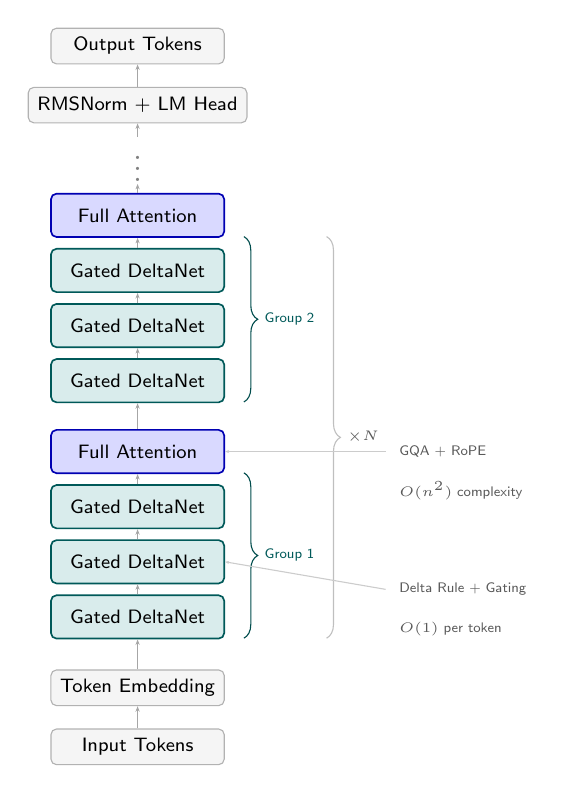
\begin{tikzpicture}[
    gdnblock/.style={rectangle, draw=teal!70!black, fill=teal!15, minimum width=2.2cm, minimum height=0.55cm, font=\scriptsize\sffamily, rounded corners=2pt, line width=0.6pt},
    fullblock/.style={rectangle, draw=blue!70!black, fill=blue!15, minimum width=2.2cm, minimum height=0.55cm, font=\scriptsize\sffamily, rounded corners=2pt, line width=0.6pt},
    ioblock/.style={rectangle, draw=gray!60, fill=gray!8, minimum width=2.2cm, minimum height=0.45cm, font=\scriptsize\sffamily, rounded corners=2pt},
    arr/.style={-{Stealth[length=2pt]}, gray!70, line width=0.5pt},
    brace/.style={decorate, decoration={brace, amplitude=5pt, mirror}},
    lbl/.style={font=\tiny\sffamily, text=gray!70!black},
]

% Input/Output
\node[ioblock] (input) at (0, 0) {Input Tokens};
\node[ioblock] (embed) at (0, 0.75) {Token Embedding};

% Layer stack - Group 1
\node[gdnblock] (l1) at (0, 1.65) {Gated DeltaNet};
\node[gdnblock] (l2) at (0, 2.35) {Gated DeltaNet};
\node[gdnblock] (l3) at (0, 3.05) {Gated DeltaNet};
\node[fullblock] (l4) at (0, 3.75) {Full Attention};

% Layer stack - Group 2
\node[gdnblock] (l5) at (0, 4.65) {Gated DeltaNet};
\node[gdnblock] (l6) at (0, 5.35) {Gated DeltaNet};
\node[gdnblock] (l7) at (0, 6.05) {Gated DeltaNet};
\node[fullblock] (l8) at (0, 6.75) {Full Attention};

% Dots
\node[font=\large, text=gray] at (0, 7.45) {$\vdots$};

\node[ioblock] (norm) at (0, 8.15) {RMSNorm + LM Head};
\node[ioblock] (output) at (0, 8.90) {Output Tokens};

% Arrows
\draw[arr] (input) -- (embed);
\draw[arr] (embed) -- (l1);
\draw[arr] (l1) -- (l2);
\draw[arr] (l2) -- (l3);
\draw[arr] (l3) -- (l4);
\draw[arr] (l4) -- (l5);
\draw[arr] (l5) -- (l6);
\draw[arr] (l6) -- (l7);
\draw[arr] (l7) -- (l8);
\draw[arr] (l8) -- ++(0, 0.4);
\draw[arr] (0, 7.75) -- (norm);
\draw[arr] (norm) -- (output);

% Braces for groups
\draw[brace, teal!60!black] (1.35, 1.38) -- (1.35, 3.48)
  node[midway, right=4pt, lbl, text=teal!70!black] {Group 1};
\draw[brace, teal!60!black] (1.35, 4.38) -- (1.35, 6.48)
  node[midway, right=4pt, lbl, text=teal!70!black] {Group 2};

% Repeat label
\draw[brace, gray!50] (2.4, 1.38) -- (2.4, 6.48)
  node[midway, right=4pt, lbl] {$\times N$};

% Side annotations
\node[lbl, anchor=west] at (3.2, 3.75) {GQA + RoPE};
\node[lbl, anchor=west] at (3.2, 3.25) {$O(n^2)$ complexity};
\draw[-{Stealth[length=1.5pt]}, gray!40, line width=0.4pt] (3.15, 3.75) -- (l4.east);

\node[lbl, anchor=west] at (3.2, 2.0) {Delta Rule + Gating};
\node[lbl, anchor=west] at (3.2, 1.5) {$O(1)$ per token};
\draw[-{Stealth[length=1.5pt]}, gray!40, line width=0.4pt] (3.15, 2.0) -- (l2.east);

\end{tikzpicture}
\caption{Qwen3.5 hybrid attention architecture. The model interleaves Gated DeltaNet layers (linear complexity, 75\%) with full softmax attention layers (quadratic complexity, 25\%) in a fixed 3:1 ratio. $N$ depends on model size: $N{=}6$ for 2B (24 layers), $N{=}8$ for 4B and 9B (32 layers).}
\label{fig:qwen35-arch}
\end{figure}

\subsubsection{Size Variants}

We evaluate three Qwen3.5 dense model variants to study the relationship between model capacity and clinical summarization performance. Table~\ref{tab:qwen35-specs} summarizes their architectural specifications, sourced from the official HuggingFace model configurations.

\begin{table}[htbp]
\centering
\caption{Qwen3.5 architecture specifications from HuggingFace \texttt{config.json}.}
\label{tab:qwen35-specs}
\begin{tabular}{lccc}
\toprule
\textbf{Specification} & \textbf{2B} & \textbf{4B} & \textbf{9B} \\
\midrule
Layers                    & 24    & 32    & 32    \\
\quad Gated DeltaNet      & 18    & 24    & 24    \\
\quad Full Attention       & 6     & 8     & 8     \\
Hidden size               & 2,048 & 2,560 & 4,096 \\
Intermediate size         & 6,144 & 9,216 & 12,288 \\
Attention heads (full)    & 8     & 16    & 16    \\
KV heads (GQA)            & 2     & 4     & 4     \\
Head dimension            & 256   & 256   & 256   \\
Context window            & 262K  & 262K  & 262K  \\
Vocabulary size           & 248,320 & 248,320 & 248,320 \\
Activation                & SiLU  & SiLU  & SiLU  \\
Normalization             & RMSNorm & RMSNorm & RMSNorm \\
\bottomrule
\end{tabular}
\end{table}

\textbf{Qwen3.5-2B} serves as a lightweight baseline, enabling rapid iteration and establishing a lower bound on small-model performance for clinical summarization. \textbf{Qwen3.5-4B} is the primary finetuning target: its 32-layer architecture provides sufficient capacity for domain adaptation via SFT and DPO, while remaining trainable on a single consumer GPU (NVIDIA RTX 5060 Ti, 16\,GB VRAM) using 4-bit quantization. \textbf{Qwen3.5-9B} provides an upper capacity bound, enabling assessment of whether larger models yield diminishing returns relative to their increased resource requirements.

All Qwen3.5 models are instruction-tuned by default, supporting structured prompt formats with system/user/assistant roles. This capability is critical for the Chain-of-Verification pipeline (Section~\ref{subsec:cove}), which requires multi-step structured reasoning with explicit output formatting.

\subsection{BioMistral Family}
\label{subsec:biomistral}

To investigate whether biomedical domain knowledge provides an advantage over general-purpose instruction-tuning for clinical summarization, we include two models from the BioMistral family~\cite{labrak2024biomistral}.

\subsubsection{Architecture}

BioMistral-7B is built upon Mistral-7B~\cite{jiang2023mistral}, a 7-billion-parameter decoder-only Transformer featuring two key architectural innovations over the vanilla Transformer:

\begin{itemize}
    \item \textbf{Grouped-Query Attention (GQA)}: 32 query heads share 8 key-value groups, reducing KV-cache memory by 4$\times$ compared to standard multi-head attention while maintaining comparable quality.
    \item \textbf{Sliding Window Attention (SWA)}: Each layer attends to the most recent 4,096 tokens rather than the full sequence, yielding linear memory scaling for long documents while relying on information propagation through stacked layers for long-range dependencies.
\end{itemize}

The biomedical adaptation was achieved through continued pretraining on a corpus sourced from PubMed Central, injecting specialized biomedical vocabulary and clinical reasoning patterns into the general-purpose Mistral foundation.

\subsubsection{SLERP Variant}

BioMistral-7B-SLERP is a model-merged variant created using Spherical Linear Interpolation (SLERP) via MergeKit~\cite{labrak2024biomistral}. Unlike standard linear weight averaging, SLERP treats model parameters as vectors on a hypersphere and computes the shortest arc between the two parent models (BioMistral-7B and Mistral-7B-Instruct-v0.1), thereby preserving the geometric structure of the weight space. The merge uses layer-specific interpolation parameters: attention layers favor the biomedical model while MLP layers retain more of the general instruction-following capability. The SLERP variant is included to test whether this hybrid merging strategy yields better clinical summarization than the pure domain-adapted model.

\subsubsection{Limitations for Inference-Time Verification}

Both BioMistral variants are \textbf{excluded from Chain-of-Verification experiments} due to an architectural limitation: BioMistral was pretrained for biomedical text generation but not instruction-tuned for multi-step structured reasoning. In our experiments, the models exhibited five failure modes when presented with CoVe prompts:

\begin{enumerate}
    \item Token-dump drafts (comma-separated fragments instead of coherent summaries)
    \item Trivially copied questions (verbatim source text instead of verification questions)
    \item Missing CONFIRMED/CONTRADICTED/UNVERIFIABLE structure
    \item Absent two-part output format (summary + verification)
    \item Amplified hallucinations (fabricated procedures not present in source)
\end{enumerate}

These failures confirm that CoVe requires instruction-following capability as a prerequisite, and domain-specific knowledge alone is insufficient. BioMistral models are therefore evaluated only on zero-shot and few-shot baselines.

\subsection{Quantization and Deployment}
\label{subsec:quantization}

All experiments are conducted on a single NVIDIA RTX 5060 Ti GPU with 16\,GB VRAM, necessitating aggressive quantization for models exceeding 4 billion parameters. We employ three quantization strategies matched to the inference and training backends:

\begin{enumerate}
    \item \textbf{GGUF Q8\_0} (Ollama): 8-bit quantization in the GGUF format, used for Qwen3.5 inference via the Ollama runtime. This format provides near-lossless quality with approximately 50\% memory reduction relative to FP16.

    \item \textbf{bitsandbytes 8-bit} (HuggingFace Transformers): Dynamic 8-bit quantization applied to BioMistral models during inference, enabling 7B-parameter models to fit within 16\,GB VRAM through the HuggingFace \texttt{load\_in\_8bit} API.

    \item \textbf{NF4 4-bit via QLoRA}~\cite{dettmers2023qlora} (Unsloth): 4-bit NormalFloat quantization used exclusively for finetuning Qwen3.5-4B. Combined with Low-Rank Adaptation (LoRA)~\cite{hu2022lora} at rank $r{=}32$ and scaling factor $\alpha{=}64$, this enables SFT and DPO training within 12--14\,GB VRAM while maintaining training stability.
\end{enumerate}

Table~\ref{tab:model-summary} provides a consolidated view of all five models, their deployment configurations, and applicable experimental techniques.

\begin{table}[htbp]
\centering
\caption{Summary of models, deployment configurations, and applicable techniques. FT = Finetuning target.}
\label{tab:model-summary}
\begin{tabular}{llclcl}
\toprule
\textbf{Model} & \textbf{Params} & \textbf{Backend} & \textbf{Quant.} & \textbf{VRAM} & \textbf{Techniques} \\
\midrule
Qwen3.5-2B       & 2B  & Ollama       & Q8\_0  & $\sim$2.5\,GB & ZS, FS, CoVe \\
Qwen3.5-4B       & 4B  & Ollama       & Q8\_0  & $\sim$5\,GB   & ZS, FS, CoVe \\
Qwen3.5-4B (FT)  & 4B  & Unsloth      & NF4    & $\sim$12\,GB  & SFT, DPO, SW-DPO \\
Qwen3.5-9B       & 9B  & Ollama       & Q8\_0  & $\sim$10\,GB  & ZS, FS, CoVe \\
BioMistral-7B    & 7B  & HF Transf.   & 8-bit  & $\sim$10\,GB  & ZS, FS \\
BioMistral-SLERP & 7B  & HF Transf.   & 8-bit  & $\sim$10\,GB  & ZS, FS \\
\bottomrule
\end{tabular}
\end{table}



% ── 3.3 EXPERIMENTAL PIPELINE ────────────────────────────────────────────────
\section{Experimental Pipeline}
\label{sec:pipeline}

% Overview paragraph describing the progressive experimentation strategy
% TODO: Write brief overview
% Content: The pipeline progresses from simple inference-time methods to
% training-time alignment, with each stage building on insights from the
% previous one. This design enables systematic isolation of each technique's
% contribution and identifies the most effective combination.

\subsection{Baseline Inference (Zero-Shot)}
\label{subsec:baseline}
% TODO: Write baseline methodology
% Content to cover:
%   - Zero-shot prompting: single instruction prompt → model generates BHC summary
%   - Prompt template design (standardized across all 5 models)
%   - 5 models × 3 token ranges × 500 samples = 7,500 total predictions
%   - Auto-checkpoint every 10 samples for crash recovery
%   - Purpose: establish performance floor for each model

\subsection{Few-Shot Prompting}
\label{subsec:fewshot}
% TODO: Write few-shot methodology
% Content to cover:
%   - 3 configurations: 1-shot, 5-shot, 10-shot
%   - Example selection strategy:
%     · 1-shot: longest example (index 36) for maximum context
%     · 5-shot: 5 shortest examples (fits context window)
%     · 10-shot: 10 shortest examples
%   - 5 models × 3 shot counts × 3 ranges = 45 experiment runs
%   - Purpose: measure whether in-context examples improve faithfulness

\subsection{Chain-of-Verification (CoVe)}
\label{subsec:cove}
% TODO: Write CoVe implementation details
% Content to cover:
%   - Based on Dhuliawala et al. (2023)
%   - 3-step pipeline (3 LLM calls per sample):
%     · Step 1 (DRAFT): baseline prompt → initial summary (may hallucinate)
%     · Step 2 (PLAN): draft + context → N verification questions
%     · Step 3 (VERIFY+REFINE): context + questions only → verified summary
%   - Design choice: Option C — plan sees draft (grounds questions in actual
%     claims), verify+refine does NOT see draft (prevents hallucination leakage)
%   - n_questions = 5 (configurable via YAML)
%   - 6-pattern regex cascade for extracting corrected summary from model output
%   - Model compatibility:
%     · Qwen3.5-2B/4B/9B: compatible (strong instruction-following)
%     · BioMistral-7B/SLERP: excluded (5 documented failure modes:
%       token dump drafts, trivial questions, no verification structure)
%   - 3 Qwen models × 3 ranges = 9 experiment runs
%   - Include: Figure of the 3-step CoVe pipeline
%   - Cite: Dhuliawala et al. (2023)

\subsection{Supervised Fine-Tuning (SFT)}
\label{subsec:sft}
% TODO: Write SFT methodology
% Content to cover:
%   - Purpose: domain adaptation — teach clinical format and medical vocabulary
%   - Target model: Qwen3.5-4B (selected based on baseline performance vs VRAM)
%   - Framework: Unsloth + QLoRA (4-bit NF4 quantization)
%   - LoRA configuration:
%     · Rank r=32, alpha=64 (2× rank, standard ratio)
%     · Target modules: all 7 linear layers (q/k/v/o/gate/up/down_proj)
%     · Dropout: 0 (standard for QLoRA)
%   - Training hyperparameters:
%     · Effective batch size: 16 (per_device=2 × gradient_accumulation=8)
%     · Learning rate: 2e-4 (cosine scheduler, 5% warmup)
%     · Epochs: 3
%     · Weight decay: 0.01
%     · Max sequence length: 4,096
%     · bf16 precision
%   - Data: 28,500 train / 1,500 eval (from 30K extracted SFT data)
%   - Training safeguards:
%     · Checkpoint every ~50 optimizer steps (crash recovery)
%     · load_best_model_at_end=True (eval_loss)
%     · Persistent logging: training.log + training_metrics.csv
%   - Estimated training time: ~30-50 hours on RTX 5060 Ti 16GB
%   - Include: Table of SFT training hyperparameters
%   - Cite: Dettmers et al. (2023) for QLoRA, Hu et al. (2022) for LoRA

\subsection{Direct Preference Optimization (DPO)}
\label{subsec:dpo}
% TODO: Write DPO methodology
% Content to cover:
%   - Purpose: preference alignment — teach model to prefer faithful over
%     hallucinated summaries
%   - Motivation from literature:
%     · Tian et al. (ICLR 2024): 40% medical hallucination reduction via FactTune
%     · F-DPO (Chaduvula et al., arXiv 2026): demonstrated that factuality-
%       conditioned margins in DPO significantly improve hallucination reduction.
%       This work directly motivated our application of DPO and the extension
%       to severity-weighted margins (SW-DPO).
%   - DPO loss formulation (key equation):
%     \begin{equation}
%       \mathcal{L}_{\text{DPO}} = -\log \sigma \left( \beta \cdot
%         \left[ \log \frac{\pi_\theta(y_w|x)}{\pi_{\text{ref}}(y_w|x)}
%              - \log \frac{\pi_\theta(y_l|x)}{\pi_{\text{ref}}(y_l|x)}
%         \right] \right)
%     \end{equation}
%     where y_w = chosen (faithful), y_l = rejected (hallucinated), β = temperature
%   - Data: 100 golden expert pairs from Hegselmann et al. (CHIL 2024)
%   - 3-way size ablation: 10 / 50 / 100 pairs (nested subsets, seed=42)
%     to study the effect of expert data scale
%   - Training configuration:
%     · Base model: SFT checkpoint (from Section 3.3.4)
%     · per_device_batch_size=1, gradient_accumulation=16
%     · Learning rate: 5e-6 (much lower than SFT)
%     · β = 0.1 (DPO temperature)
%     · Epochs: 1 (DPO overfits fast on small datasets)
%     · max_length=2048, max_prompt_length=1536
%   - Overfitting monitoring: reward_accuracy (target: 0.65-0.85, stop if >0.90)
%   - This serves as the control/replication baseline for the SW-DPO experiment
%   - Include: Table of DPO ablation runs (10/50/100 pairs)
%   - Cite: Rafailov et al. (2023) for DPO, Tian et al. (2024) for FactTune,
%     Chaduvula et al. (2026) for F-DPO

\subsection{Severity-Weighted DPO (SW-DPO)}
\label{subsec:swdpo}
% TODO: ⭐ CORE CONTRIBUTION — write the novel method
% Content to cover:
%   - Motivation: standard DPO treats all hallucinations equally, but in
%     clinical settings, fabricating a medication (e.g., wrong drug/dose) is
%     far more dangerous than a minor word-level imprecision. F-DPO
%     (Chaduvula et al., 2026) showed that factuality-conditioned margins
%     improve DPO, but used generic factuality scores. We extend this idea
%     with domain-specific clinical severity from expert annotations.
%
%   - NCC MERP Severity Weight Mapping:
%     · The National Coordinating Council for Medication Error Reporting and
%       Prevention (NCC MERP) provides a standardized severity index for
%       categorizing medication errors by patient harm potential.
%     · We map each of the 11 hallucination categories from Hegselmann et al.
%       to severity weights derived from the NCC MERP framework:
%       - contradicted_fact: 5.0 (direct contradiction → wrong treatment risk)
%       - medication_unsupported: 4.0 (wrong drug/dose → adverse events)
%       - condition_unsupported: 3.5 (wrong diagnosis → wrong treatment plan)
%       - procedure_unsupported: 3.0 (wrong procedure → misleading follow-up)
%       - number_unsupported: 3.0 (wrong lab value → clinical decisions)
%       - time_unsupported: 2.0 (wrong timing → scheduling errors)
%       - location_unsupported: 2.0 (wrong body part → usually obvious)
%       - name_unsupported: 1.5 (wrong specialist → low clinical impact)
%       - word_unsupported: 1.0 (stylistic/word-level → minimal risk)
%       - other_unsupported: 1.0 (catch-all → minimal impact)
%     · No additional human annotation needed — weights are deterministically
%       derived from the existing expert span annotations + NCC MERP.
%     · Include: Table of severity weight mapping with clinical rationale
%
%   - Per-sample severity score computation:
%     · severity(y_l) = Σ weight(category_i) × count(category_i)
%       for all hallucination spans in the rejected response
%     · Normalized: norm_sev = severity(y_l) / max_severity_in_dataset → [0, 1]
%
%   - SW-DPO loss formulation (KEY EQUATION):
%     \begin{equation}
%       \mathcal{L}_{\text{SW-DPO}} = -\log \sigma \left( \beta \cdot
%         \left[ \log \frac{\pi_\theta(y_w|x)}{\pi_{\text{ref}}(y_w|x)}
%              - \log \frac{\pi_\theta(y_l|x)}{\pi_{\text{ref}}(y_l|x)}
%         \right] - \alpha \cdot s_{\text{norm}}(y_l) \right)
%     \end{equation}
%     where:
%       · α ∈ {0.5, 1.0, 2.0} — margin strength hyperparameter
%       · s_norm(y_l) ∈ [0, 1] — min-max normalized severity score
%       · Higher severity → larger margin → stronger gradient push
%
%   - 3-way severity ablation (all using 100 golden pairs):
%     · DPO-Uniform: α=0, standard DPO (replication baseline from Sec 3.3.5)
%     · SW-DPO-Binary: margin = α × {0 if no hallucination, 1 if any}
%       (tests whether ANY severity signal helps)
%     · SW-DPO-Severity: margin = α × normalized severity score
%       (tests whether GRADED severity helps)
%   - Implementation: subclass TRL DPOTrainer, override get_batch_loss_metrics()
%     to inject per-sample severity margins from the dataset
%   - α hyperparameter sweep: {0.5, 1.0, 2.0} on 10 validation pairs
%   - Include: Ablation experiment table, SW-DPO loss equation (numbered)
%   - Cite: NCC MERP (2001), Chaduvula et al. (2026) for F-DPO,
%     Hegselmann et al. (2024) for expert annotations

\subsection{SW-DPO + CoVe Stacking}
\label{subsec:stacking}
% TODO: Write combined method description
% Content to cover:
%   - Hypothesis: training-time alignment (SW-DPO) and inference-time
%     verification (CoVe) address hallucination through complementary mechanisms:
%     · SW-DPO: reduces the model's internal tendency to generate high-severity
%       hallucinations (changes model weights)
%     · CoVe: catches remaining hallucinations through explicit verification
%       and correction (external post-generation check)
%   - Pipeline: best SW-DPO checkpoint → run through 3-step CoVe pipeline
%   - Expected synergy: SW-DPO provides a better "draft" (Step 1 of CoVe),
%     CoVe then corrects any remaining errors
%   - Evaluation: same metrics as individual methods, enabling direct comparison
%   - Include: Figure showing the stacked pipeline

\subsection{Experimental Configuration Summary}
\label{subsec:ablation-summary}

Table~\ref{tab:ablation-summary} provides an overview of the seven experimental configurations evaluated in this thesis, organized in order of increasing methodological complexity. Each configuration is designed to isolate the contribution of a specific technique, enabling progressive comparison from the baseline through the full stacked pipeline.

\begin{table}[htbp]
\centering
\caption{Summary of experimental configurations. Each row adds one technique to measure its incremental contribution to summarization quality and faithfulness.}
\label{tab:ablation-summary}
\small
\begin{tabular}{llllp{4.5cm}}
\toprule
\textbf{Config} & \textbf{Training} & \textbf{Inference} & \textbf{Models} & \textbf{What It Tests} \\
\midrule
Baseline     & ---          & Zero-shot      & All 5   & Performance floor \\
Few-shot     & ---          & $k$-shot       & All 5   & In-context learning effect \\
CoVe         & ---          & 3-step verify  & Qwen only & Inference-time verification \\
\midrule
SFT          & 30K pairs    & Zero-shot      & Qwen 4B & Domain adaptation \\
DPO-Uniform  & 100 expert   & Zero-shot      & Qwen 4B & Preference alignment \\
SW-DPO       & 100 expert   & Zero-shot      & Qwen 4B & Severity-weighted margins \\
SW-DPO+CoVe  & 100 expert   & 3-step verify  & Qwen 4B & Synergy of both methods \\
\bottomrule
\end{tabular}
\end{table}

% ── 3.4 EVALUATION FRAMEWORK ────────────────────────────────────────────────
\section{Evaluation Framework}
\label{sec:evaluation}


Evaluation of clinical summarization requires measuring two complementary properties: (i) whether the generated summary captures the essential clinical information present in the reference summary (\textit{completeness}), and (ii) whether every claim in the generated summary is supported by the source clinical notes (\textit{faithfulness}). These two axes correspond to distinct comparison targets: completeness metrics compare the predicted summary $P$ against the labeled reference summary $L$ written by a physician, while faithfulness metrics compare $P$ against the source clinical context $C$.

\subsection{Completeness Metrics (P vs.\ L)}
\label{subsec:completeness}

Completeness metrics quantify the information overlap between a model-generated summary $P$ and the physician-written reference $L$. We report three complementary metrics:

\textbf{ROUGE-1 F1}~\cite{lin2004rouge} computes the harmonic mean of unigram precision and recall between $P$ and $L$. Despite its simplicity, ROUGE-1 remains the most widely reported metric in clinical summarization research, providing a reliable proxy for surface-level content coverage. We use the \texttt{rouge-score} implementation with Porter stemming enabled.

\textbf{BLEU}~\cite{papineni2002bleu} is a precision-oriented metric that measures n-gram overlap (up to 4-grams) between $P$ and $L$, with a brevity penalty to discourage overly short outputs. While originally designed for machine translation, BLEU complements ROUGE by emphasizing precision (whether generated n-grams appear in the reference) rather than recall. We report sentence-level BLEU scores on a 0--100 scale using SacreBLEU.

\textbf{BERTScore F1}~\cite{zhang2020bertscore} moves beyond surface-level token matching by computing cosine similarity between contextual token embeddings from a pretrained language model. Each token in $P$ is greedily matched to its most similar token in $L$ (and vice versa), yielding embedding-based precision, recall, and F1 scores. This captures semantic equivalence that n-gram metrics miss---for example, recognizing that ``cardiac arrest'' and ``heart attack'' convey similar clinical meaning. We use the DeBERTa-XLarge-MNLI variant recommended by the authors.

\subsection{Faithfulness Metrics (P vs.\ C)}
\label{subsec:faithfulness}

Faithfulness metrics detect hallucinations by evaluating whether each claim in the generated summary $P$ is supported by the source clinical notes $C$. Unlike completeness metrics, faithfulness evaluation does not use the reference summary---a summary can be faithful (all facts are supported by the source) without being complete (some important facts are omitted). We employ two NLI-based metrics that represent the current state of the art in automated factual consistency evaluation.

\subsubsection{SummaC}

SummaC~\cite{laban2022summac} addresses a fundamental granularity mismatch: NLI models are trained on sentence-level premise-hypothesis pairs, yet factual consistency must be evaluated at the document level. Rather than feeding entire documents to an NLI model (which degrades performance), SummaC decomposes the evaluation into sentence-level comparisons.

The algorithm operates as follows. Given a source document $C$ with $M$ sentences and a summary $P$ with $N$ sentences, SummaC first constructs an $M \times N$ NLI pair matrix by running each $(C_i, P_j)$ pair through an NLI model and extracting the entailment probability $E_{ij}$. Two aggregation strategies then convert this matrix into a single consistency score:

\begin{itemize}
    \item \textbf{SummaC-ZS} (Zero-Shot): For each summary sentence $P_j$, the maximum entailment score across all document sentences is retained (identifying the strongest supporting evidence). The final score is the mean of these maxima:
    \begin{equation}
        \text{SummaC-ZS} = \frac{1}{N} \sum_{j=1}^{N} \max_{i} E_{ij}
        \label{eq:summac-zs}
    \end{equation}

    \item \textbf{SummaC-Conv} (Convolutional): Rather than relying on the maximum (which is sensitive to outliers), this variant bins the entailment score distribution for each summary sentence into a fixed-size histogram and applies a learned 1-D convolution layer to produce a per-sentence score. The convolution layer is trained on the FactCC synthetic dataset~\cite{laban2022summac}.
\end{itemize}

We use the \texttt{vitc} NLI model variant (ALBERT-XLarge trained on VitaminC + MNLI), which achieved the highest benchmark performance in the original paper at 74.4\% balanced accuracy across six datasets. SummaC-ZS scores range from $[-1, +1]$ and SummaC-Conv scores range from $[0, 1]$.

\subsubsection{AlignScore}

AlignScore~\cite{zha2023alignscore} takes a fundamentally different approach by training a unified alignment function on 4.7 million examples spanning seven NLP tasks (NLI, QA, paraphrasing, fact verification, information retrieval, semantic similarity, and summarization). This diverse training enables the model to capture a broader range of factual consistency signals than NLI-only metrics.

At inference time, AlignScore addresses the input length limitation of its RoBERTa backbone (512 tokens) through a chunk-based evaluation strategy:

\begin{enumerate}
    \item The source context $C$ is split at sentence boundaries into chunks of approximately 350 tokens each, ensuring that each chunk concatenated with a claim sentence fits within the 512-token limit.
    \item The summary $P$ is split into individual sentences $\{P_j\}$.
    \item Each claim sentence $P_j$ is evaluated against all context chunks, and the maximum alignment score is retained.
    \item The final score is the mean of the per-sentence maxima:
\end{enumerate}
\begin{equation}
    \text{AlignScore}(C, P) = \frac{1}{N} \sum_{j=1}^{N} \max_{i} \text{align}(C'_i, P_j)
    \label{eq:alignscore}
\end{equation}
where $\{C'_i\}$ are the context chunks and $\text{align}(\cdot)$ is the probability of the \textsc{aligned} label from the 3-way classification head. We use the AlignScore-large variant (RoBERTa-Large, 355M parameters) in \texttt{nli\_sp} evaluation mode. Scores range from $[0, 1]$.

The chunk-level strategy is critical for clinical summarization, where source documents (discharge notes) frequently exceed 1,000 tokens. AlignScore's coarser chunking preserves paragraph-level semantic context that would be lost in SummaC's sentence-level decomposition, making the two metrics complementary.

\subsubsection{Metric Summary}

Table~\ref{tab:eval-metrics} consolidates the properties of all evaluation metrics used in this thesis.

\begin{table}[htbp]
\centering
\caption{Summary of evaluation metrics. $P$ = predicted summary, $L$ = labeled reference, $C$ = source clinical notes.}
\label{tab:eval-metrics}
\begin{tabular}{llcl}
\toprule
\textbf{Metric} & \textbf{Comparison} & \textbf{Range} & \textbf{Aspect} \\
\midrule
ROUGE-1 F1   & $P$ vs.\ $L$ & $[0, 1]$    & N-gram recall \\
BLEU         & $P$ vs.\ $L$ & $[0, 100]$  & N-gram precision \\
BERTScore F1 & $P$ vs.\ $L$ & $[0, 1]$    & Semantic similarity \\
\midrule
SummaC-ZS    & $P$ vs.\ $C$ & $[-1, +1]$  & NLI entailment \\
SummaC-Conv  & $P$ vs.\ $C$ & $[0, 1]$    & NLI entailment \\
AlignScore   & $P$ vs.\ $C$ & $[0, 1]$    & Unified alignment \\
\bottomrule
\end{tabular}
\end{table}

\subsection{Category-Level Hallucination Analysis}
\label{subsec:category-eval}
% TODO: Write category-level evaluation description (deferred pending experimental results)
% Content to cover:
%   - Purpose: go beyond aggregate scores to understand WHICH types of
%     hallucinations each method reduces
%   - New metric: High-Severity Hallucination Rate
%     · Breakdown by hallucination category (medication, condition, contradicted_fact)
%   - Per-category comparison across all methods
%   - Particularly relevant for SW-DPO evaluation: does severity weighting
%     specifically reduce dangerous errors more than uniform DPO?
%   - Include: description of how category-level errors are identified and counted


% ── 3.5 HARDWARE AND SOFTWARE ───────────────────────────────────────────────
\section{Hardware and Software Environment}
\label{sec:hardware}
% TODO: Write experimental setup description
% Content to cover:
%   - Hardware:
%     · GPU: NVIDIA RTX 5060 Ti 16GB VRAM (Blackwell architecture)
%     · CPU: AMD Ryzen 7 5700X
%     · RAM: 32 GB
%   - Software stack:
%     · OS: Ubuntu Server 26.04 LTS
%     · CUDA: 12.8 (PyTorch cu128)
%     · Python: 3.11
%     · Key libraries: PyTorch 2.10, Unsloth, TRL, HuggingFace Transformers,
%       PEFT, bitsandbytes, XFormers
%   - Environment setup:
%     · 3 separate conda environments due to irreconcilable dependency conflicts
%       between SummaC, AlignScore, and the main training stack
%     · vinhthesis: main env (inference + evaluation + finetuning)
%     · eval_summac: SummaC evaluation
%     · eval_align: AlignScore evaluation
%   - Include: Table of hardware and key software versions


% ====================================================================
%  CHAPTER 4: RESULTS AND EVALUATION
% ====================================================================
\chapter{Results and Evaluation}
\label{ch:results}

% ~10-15 pages. Tables, figures, analysis.

\section{Baseline and Few-Shot Results}
\label{sec:baseline-results}
% TODO: Present baseline performance
%   - 5 models × 3 ranges completeness + faithfulness tables
%   - Model ranking analysis
%   - Few-shot (1/5/10) improvement analysis
%   - Per-range performance variation (short vs medium vs long)
%
% QUESTION FOR YOU: How many tables do you envision here?
% One big table or separate tables per metric category?

\section{Chain-of-Verification Results}
\label{sec:cove-results}
% TODO: CoVe performance
%   - Qwen3.5 2B/4B/9B × 3 ranges
%   - Comparison with baseline and few-shot
%   - BioMistral failure analysis

\section{SFT Results}
\label{sec:sft-results}
% TODO: Domain adaptation impact
%   - Training curves (loss, eval_loss)
%   - SFT model vs baseline Qwen3.5-4B comparison
%   - Completeness + faithfulness changes

\section{DPO Results}
\label{sec:dpo-results}

\subsection{Size Ablation (10/50/100 Pairs)}
\label{subsec:dpo-size}
% TODO: [PLACEHOLDER — experiments pending]
%   - DPO-Uniform performance across 3 dataset sizes
%   - Data efficiency analysis

\subsection{SW-DPO Severity Ablation}
\label{subsec:swdpo-results}
% TODO: [PLACEHOLDER — experiments pending] ⭐ KEY RESULTS
%   - Uniform vs Binary vs Severity comparison
%   - Category-level hallucination breakdown
%   - High-severity error reduction rates
%   - α hyperparameter sensitivity

\section{Combined SW-DPO + CoVe Results}
\label{sec:combined-results}
% TODO: [PLACEHOLDER — experiments pending]
%   - Stacking vs individual methods
%   - Synergistic effect analysis

\section{Comprehensive Comparison}
\label{sec:comparison}
% TODO: Final comparison table
%   - All methods: Baseline → Few-Shot → CoVe → SFT → DPO-U → SW-DPO → SW-DPO+CoVe
%   - Faithfulness, Completeness, High-Severity metrics
%   - Statistical significance tests
%   - Visualization: bar charts, heatmaps

\section{Discussion}
\label{sec:discussion}
% TODO: Interpret results
%   - Why does severity weighting help (or not)?
%   - Why does stacking work (or not)?
%   - Limitations: task mismatch, small DPO dataset, single GPU
%   - Comparison with published results (Tian et al., Hegselmann et al.)
%
% QUESTION FOR YOU: Should Discussion be its own chapter (Chapter 5)
% or a section within Results (as I have it now)?


% ====================================================================
%  CHAPTER 5: CONCLUSION AND FUTURE WORK
% ====================================================================
\chapter{Conclusion and Future Work}
\label{ch:conclusion}

% ~3-5 pages

\section{Summary of Findings}
\label{sec:summary}
% TODO: Summarize key findings
%   - Answer each research question
%   - Highlight SW-DPO contribution

\section{Contributions Revisited}
\label{sec:contributions-revisited}
% TODO: Restate contributions with evidence
%   - C1: SW-DPO effectiveness
%   - C2: Stacking synergy
%   - C3: Benchmark results
%   - C4: Category-level evaluation

\section{Limitations}
\label{sec:limitations}
% TODO: Honest limitations
%   - Single GPU (RTX 5060 Ti 16GB) — limited model scale
%   - 100 expert pairs — small dataset for DPO
%   - Task mismatch (BHC→patient vs notes→BHC)
%   - NCC MERP weights are assigned heuristically
%   - Evaluation on MIMIC-IV only (no external validation)

\section{Future Work}
\label{sec:future-work}
% TODO: Future directions
%   - Multi-agent debate for verification
%   - DoLa decoding integration
%   - Larger expert-annotated datasets
%   - Multi-institution validation
%   - Deployment in clinical decision support systems
%   - Extension to other clinical NLP tasks


% ====================================================================
%  REFERENCES
% ====================================================================
\bibliographystyle{IEEEtran}
\bibliography{references}


% ====================================================================
%  APPENDICES
% ====================================================================
\appendix

\chapter{Prompt Templates}
\label{app:prompts}
% TODO: Include baseline, few-shot, CoVe plan, CoVe verify+refine prompts

\chapter{Detailed Experimental Results}
\label{app:detailed-results}
% TODO: Full per-range, per-model result tables

\chapter{Hallucination Category Examples}
\label{app:hallucination-examples}
% TODO: Example hallucinations from each of the 11 categories

\end{document}
